% These are the lecture notes for my CSC1101 course Fall 2016
% at CityTech. They are based largely on How To Think Like A
% Computer Scientist. See last slide for reference information.

% Feel free to edit these slides and use them for your own courses.
% HOWEVER DO NOT REMOVE THESE LINES!
% Email me at: awood [at] citytech.cuny.edu
% or at: awood [at] gradcenter.cuny.edu

\documentclass{beamer}

\usepackage{tikz}
\usetikzlibrary{calc}
\usepackage{alltt}
\usepackage{forest}
\usepackage{verbatim}


\setbeamertemplate{footline}[frame number]
\setbeamertemplate{navigation symbols}{} 

\newtheorem{thm}{Theorem}[section]
\newtheorem{lem}{Lemma}
\newtheorem{cl}{Claim}
\newtheorem{cor}{Corollary}[section]
\newtheorem{conj}{Conjecture}
\newtheorem{quest}{Question}
\newtheorem{defn}{Definition}[section]
\newtheorem{obs}{Observation}[section]
\newtheorem{exam}{Example}


\mode<presentation>
{
%  \usetheme{default}
  \setbeamercovered{invisible}
}


\usepackage[english]{babel}
\usepackage[latin1]{inputenc}
\usepackage{times}
\usepackage[T1]{fontenc}
\usepackage{stmaryrd}

%\usetheme{default}
%\usetheme{AnnArbor}
%\usetheme{Antibes}
%\usetheme{Bergen}
%\usetheme{Berkeley}
%\usetheme{Berlin}
%\usetheme{Boadilla}
%\usetheme{CambridgeUS}
%\usetheme{Copenhagen}
%\usetheme{Darmstadt}
%\usetheme{Dresden}
%\usetheme{Frankfurt}
%\usetheme{Goettingen}
%\usetheme{Hannover}
%\usetheme{Ilmenau}
%\usetheme{JuanLesPins}
%\usetheme{Luebeck}
%\usetheme{Madrid}
%\usetheme{Malmoe}
%\usetheme{Marburg}
%\usetheme{Montpellier}
%\usetheme{PaloAlto}
%\usetheme{Pittsburgh}
%\usetheme{Rochester}
\usetheme{Singapore}
%\usetheme{Szeged}
%\usetheme{Warsaw}

%\usecolortheme{default}
%\usecolortheme{albatross}
\usecolortheme{beaver}
%\usecolortheme{beetle}
%\usecolortheme{crane}
%\usecolortheme{dolphin}
%\usecolortheme{dove} % grey, white, yellow
%\usecolortheme{fly} %grey, yellow
%\usecolortheme{lily} %white, yellow, blue
%\usecolortheme{orchid}
%\usecolortheme{rose}
%\usecolortheme{seagull}
%\usecolortheme{seahorse}
%\usecolortheme{whale}
%\usecolortheme{wolverine}


\title[Boolean Logic]{Python 2.7: Boolean Logic}
\subtitle{}

\author
{Lecture notes of Alexander Wood \\ \scriptsize \href{mailto:awood@citytech.cuny.edu}{awood@citytech.cuny.edu}}
\institute[CityTech]{New York City College of Technology }  

\date{}

%\beamerdefaultoverlayspecification{<+->}


\begin{document}

%%%%
\begin{frame}
  \titlepage
\end{frame}

\section{Boolean Expressions}

%%%%
\begin{frame}[fragile]
\frametitle{Boolean expressions}

A \textbf{boolean expression} is an expression which is either true or false. The values \verb|True| and \verb|False| are special values of type \verb|bool|.
\begin{figure}\centering
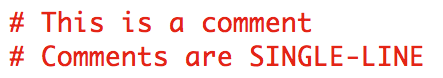
\includegraphics[scale=.8]{IMG/1.png}
\end{figure}
\end{frame}

%%%%
\begin{frame}
\frametitle{Relational operators}

There are a variety of relational operators, which tell us whether a relationship is True or False.

\vspace{4mm}
\begin{tabular}{l*{2}{l}r}
\textbf{Operator   }           & \textbf{Meaning}  \\
\hline
$>$ & Greater than  \\
$<$  & Less than  \\
$>=$  & Greater than or equal to   \\
$<=$ & Less than or equal to   \\
$==$ & Equal to\\
$!=$ & Not equal to
\end{tabular}
\end{frame}


%%%%
\begin{frame}
\frametitle{Relational operators}

\begin{figure}\centering
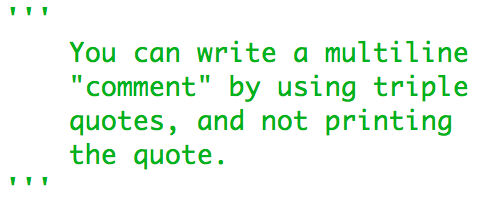
\includegraphics[scale=.8]{IMG/2.png}
\end{figure}
\end{frame}

%%%%
\begin{frame}[fragile]
\frametitle{Relational Operators}

Note that \verb|==| is used to test equality. The single equal sign, \verb|=|, is used to assign a value to a variable.
\begin{figure}\centering
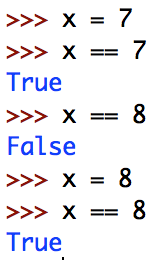
\includegraphics[scale=.8]{IMG/assign.png}
\end{figure}
\end{frame}





\section{Logical Operators}

%%%%
\begin{frame}[fragile]
\frametitle{Logical Operators}

The logical operators are \verb|and|, \verb|or|, and \verb|not|.
\begin{itemize}
\item {\alltt{x{\color{orange} and} y}} is true if BOTH \verb|x| and \verb|y| are true
\item {\alltt{x{\color{orange} or} y}} is true if EITHER \verb|x| or \verb|y| is true
\item {\alltt{{\color{orange}not} x}} negates (ie, switches) the truth value of a boolean expression
\end{itemize}
\end{frame}

%%%%
\begin{frame}
\frametitle{Logical Operators}

Remember to use parenthesis to avoid confusion about precedence!
\begin{alltt}
x > 5 {\color{orange}and} x < 6

(x > 5) {\color{orange}and} (x < 6)
\end{alltt}
\end{frame}

%%%%
\begin{frame}
\frametitle{Logical Operators}

\begin{figure}\centering
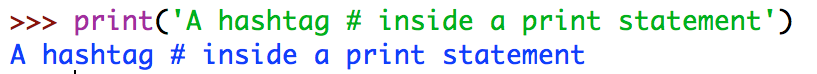
\includegraphics[scale=.8]{IMG/3.png}
\end{figure}
\end{frame}



\section{What is True?}

%%%%
\begin{frame}[fragile]
\frametitle{What is True?}

What if we type the following:
\begin{alltt}
{\color{purple}bool}({\color{green}"Hotline Bling"})
\end{alltt}
Does this  evaluate to \verb|True|, or \verb|False|? In other words, we are asking ourselves the big question: What does Python consider to be True?
\end{frame}

%%%%
\begin{frame}[fragile]
\frametitle{What is False?}

To determine what is \verb|True|, we must first determine what is \verb|False|. The following are all considered false:
\begin{verbatim}
bool:        False
null         None
integer:     0
float:       0.0
string:      ''
list:        []
tuple:       ()
dictionary:  {}
set:         set()
\end{verbatim}
Note that we have NOT covered lists, tuples, dictionaries, or sets yet in this course.
\end{frame}

%%%%
\begin{frame}[fragile]
\frametitle{What is True?}

Everything which is not \verb|False| is considered \verb|True| in Python. This is counter-intuitive and takes some getting used to, but ends up being quite useful.

\begin{figure}\centering
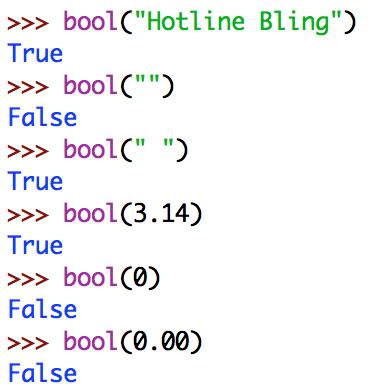
\includegraphics[scale=.8]{IMG/bool.png}
\end{figure}
\end{frame}

%%%%
\begin{frame}
\frametitle{Testing for empty data structures}

A common application of this `truthiness' definition in Python is checking for empty data structures. See the example below, which checks for an empty string.

\begin{figure}\centering
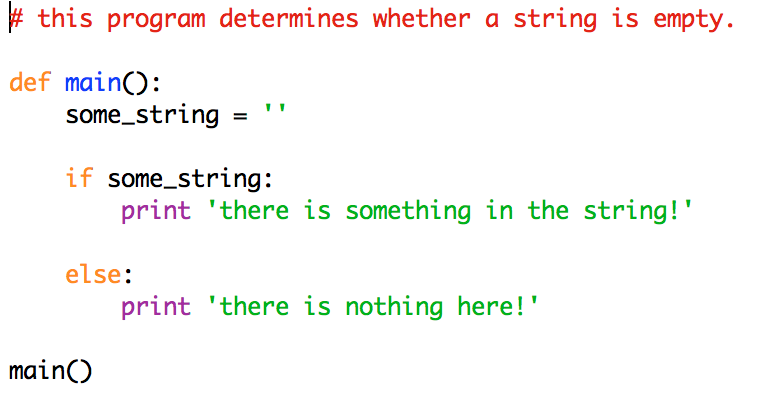
\includegraphics[scale=.7]{IMG/4.png}
\end{figure}
\end{frame}

%%%%
\begin{frame}
\frametitle{References}

\begin{itemize}
\item
\url{http://www.openbookproject.net/thinkcs/python/english2e/ch04.html}
\end{itemize}
\end{frame}
\end{document}


